\chapter{Introduction}
\label{chp:intro}

\noindent To make an unified communication solution with \gls{webrtc}, integrating \gls{webrtc} technology with traditional telephony network is the main goal of it. The term, unified communication, in this thesis means the unified solution for real time communication on the internet and on the traditional telephony network.

\section{Background and Motivation}

\par As the development of smart mobile phone industry, there are more and more people connected to the internet through smart phones. The real time communication demands is from the traditional telephony network to \gls{ip} network. There are many client applications provide real time communication service through the internet. There are two main different categories for these real time communication solution. One kind of application is like Google Hangout, it provides user a real time communication channel on the internet and require user client both using browser to communicate with each other. The other kind of application is like Skype\footnote{Skype is a freemium voice-over-IP service and instant messaging client, currently developed by the Microsoft Skype Division. The name was derived from "sky" and "peer".\cite{wiki:skype}}, it provides \gls{voip} service and let different client users(browser and physical phone) to communicate with each other.

\par However, the problem of the second category application is that users have to install some application client and request for some application credential to use the service. There are already many different applications installed on user's smart phone and desktop computer. It is hard for user to remember another application credential and install one more application for just calling.

\par The motivation of this thesis is to provide an unified communication solution for user easily to have real time conversation with the other user either on mobile phone or desktop computer. The unified communication solution should not demand user to install any client software or plugins and not ask user to remember another new credential information either.

\par The approach for that would be a web application service using user telephone number as credential and provide the user call any kind of other user no matter the other user is on his mobile phone or his computer through internet. This system will be a \gls{ott} solution integrated with \gls{webrtc} network and \gls{voip} network. The service can provide user a new real time communication way to reach other people in the world since every one is on the internet or on the phone nowadays.

\par The prototype system implemented in this thesis will provide rich multimedia real-time communication service with \gls{webrtc} network and \gls{sip} network. Some basic real-time communication application functions will be achieved, like calling mobile phone, having video conferencing, instance messaging and file sharing. And normal telephony functions will be achieved by the prototype system as well, for instance, calling phone number, receiving call from other phone number, forwarding phone and \gls{sms} messaging.

\section{Challenges}

\noindent Challenges of this thesis are mainly from two categories, research challenges and implementation challenges.

\par As research challenges, since \gls{webrtc} technology is quite new web technology and not scandalized yet, there are a lot of articles about it but they are not all relevant to the topic because different browser has different implementation on \gls{webrtc} and the implementation keeps changing with the updates of the browser. Moreover, there are not many open sourced project to support \gls{sip} on the web application. The objective is to integrate \gls{webrtc} technology with traditional telephony network, then it is necessary to do the search about the similar implementing project or application. There are no such directly communication between \gls{sip} and \gls{webrtc}. The research cases could be studied are mostly implementing one of the technology.

\par As implementation challenges, there are no similar commercial products using technology as the prototype system in this thesis in the market yet. The combination of the technologies using in the prototype system is completely new in the field. There are not so many references and documentation could be used during the development. Student who developed the system need to understand the basic and fundamental knowledge about \gls{sip} protocol and \gls{webrtc} implementation. It requires a lot of time on programming prototype test demo to evaluate the implementation solutions. Furthermore, there are many system design cases need to be considered during the development because the target integration system is traditional telephony network which requires high system stability. All the implementation source code of the prototype system to achieve the objective of unified communication solution with \gls{webrtc} is created by the student alone. Some of them are based on other third party library with some changes by the student. These development process requires student very high programming skills on some specific programming and network knowledge.

\section{Method}

\noindent The main focus of this thesis is to research about how to make an unified communication system with \gls{webrtc} technology. The approach to this goal will be studies about \gls{webrtc} and its commercial usage and also the prototype implementation to verify the prototype system design and some ideas about the way to implement this unified communication system. The approach for this goal in the thesis is to implement the prototype system and demo tests to understand the different solutions and analysis their advantages and disadvantages.

\par To achieve the goal of this thesis, the research progress will be under the Spiral development\footnote{The spiral model is a risk-driven process model generator for software projects. Based on the unique risk patterns of a given project, the spiral model guides a team to adopt elements of one or more process models, such as incremental, waterfall, or evolutionary prototyping.\cite{wiki:spiral}} and Prototyping\footnote{Software prototyping, refers to the activity of creating prototypes of software applications, i.e., incomplete versions of the software program being developed. It is an activity that can occur in software development and is comparable to prototyping as known from other fields, such as mechanical engineering or manufacturing.
A prototype typically simulates only a few aspects of, and may be completely different from, the final product.\cite{wiki:prototyping}} software development methodology. 

\par The reason to use these two software development methodologies is that this thesis is a single person project and the goal of this thesis is to figure out how to integrate one technology to exist business market. Then the Scrum development method\footnote{Scrum is an iterative and incremental agile software development framework for managing software projects and product or application development. It defines "a flexible, holistic product development strategy where a development team works as a unit to reach a common goal". It challenges assumptions of the "traditional, sequential approach" to product development. Scrum enables teams to self-organize by encouraging physical co-location or close online collaboration of all team members and daily face-to-face communication among all team members and disciplines in the project.\cite{wiki:scrum}} is not suitable for one person project since it causes too much time to discuss problem with others to get feedback and also it will cause too much plan than the research or development work load. There will not be too much continues user interaction during the research and development then it is not suitable to use Rapid application development in this thesis.

\subsection{Spiral Development}

\par Because the target network for unified communication solution is telephony network which requires high stability in the real live, using risk-driven process model like Spiral development is quite suitable in this thesis. The basic Spiral development model is shown in Figure \ref{fig:spiral}.

\begin{figure}
	\centering
    	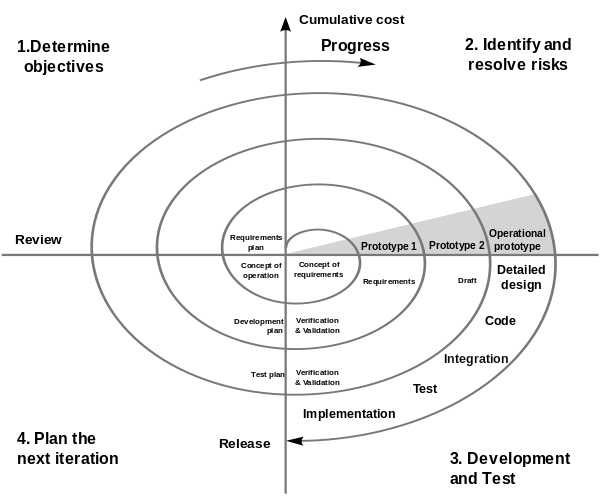
\includegraphics[width=0.70\textwidth,natwidth=610,natheight=642]{figs/Spiral_model.png}
  	\caption{Spiral Development Model}
  	\label{fig:spiral}
\end{figure}

\noindent The basic principles of Spiral Development are shown below\cite{wiki:software_method}:

\begin{itemize}[topsep=-1em,parsep=0em,itemsep=0em]
    \item Focus is on risk assessment and on minimizing project risk by breaking a project into smaller segments and providing more ease-of-change during the development process, as well as providing the opportunity to evaluate risks and weigh consideration of project continuation throughout the life cycle.
    \item "Each cycle involves a progression through the same sequence of steps, for each part of the product and for each of its levels of elaboration, from an overall concept-of-operation document down to the coding of each individual program."
    \item Each trip around the spiral traverses four basic quadrants: (1) determine objectives, alternatives, and constraints of the iteration; (2) evaluate alternatives; Identify and resolve risks; (3) develop and verify deliverables from the iteration; and (4) plan the next iteration.
    \item Begin each cycle with an identification of stakeholders and their win conditions, and end each cycle with review and commitment.
\end{itemize}

\par Like which is shown in the Figure \ref{fig:spiral}, there are four steps in each development circle. Considering the objective of the thesis, there will be several development circle regarding to the functionality of the unified communication solution for the prototype system. They are shown in the below Table \ref{tab:spiral}(Most of the evaluation and implementation explanation will be hold in later Chapters).

\begin{table}
\caption{\label{tab:spiral}: Unified Communication Solution Spiral Model}
\centering
\begin{tabular}{| p{5cm} | c | p{5cm} |}
\hline
Function & Risk Level & Evaluation Method \\ \hline
\gls{webrtc} Conversation & Low & Implement basic \gls{webrtc} with different frameworks\\ \hline
\gls{webrtc} with \gls{sip} conversation & Low & Research with different solutions in demo tests \\ \hline
\gls{webrtc} DataChannel & High & Research about \gls{webrtc} DataChannel Usage on XMS Server \\ \hline
Rich Multimedia Conversation & Low & Implement basic real time communication functions to test \\ \hline
\gls{webrtc} Browser Compatibility & Medium & Implementation tests on different browsers \\ \hline
Advanced Real-time Conversation Functions & Medium & Research and implementation tests on some advanced real time conversation functions \\
\hline
\end{tabular} 
\end{table}


\par During the prototype system development in this thesis, the risk of each function implementation is how the functionality will be integrated with telephony network in \gls{webrtc}. There are some advanced \gls{webrtc} technology which are difficult and high risk to cause more problem than the benefits of the prototype system during the development. They will be addressed during the Chapter \ref{chp:sys_design} and Chapter \ref{chp:future_work} to explain the reason why they got dropped from the prototype system and how these functions can be implemented in the fureture.

\par In the Table \ref{tab:spiral}, the order of the function lists are the same development circle order during the prototype system implementation and research of the thesis's topic. They are from the basic function which is higher priority to lower. Considering the risk level to the exist telephony \gls{voip} network and the evaluation result, some of them will not be include in the final prototype system of the thesis. But all of them are going through the four steps of Spiral development model, first to analysis the function requirement, second to evaluate the possible solution to implement the function, third to make some demo tests or prototype implementation in order to get feedback, at last to decide if this function can be included in the prototype system and plan for next function implementation.

\subsection{Prototyping}

\par Prototyping has several benefits: The software designer and implementer can get valuable feedback from the users early in the project. The client and the contractor can compare if the software made matches the software specification, according to which the software program is built. It also allows the software engineer some insight into the accuracy of initial project estimates and whether the deadlines and milestones proposed can be successfully met. The degree of completeness and the techniques used in the prototyping have been in development and debate since its proposal in the early 1970s.\cite{wiki:prototyping}

\par There will be different case studies and implementation solution demo testing in the thesis. They are helping the research about the unified communication solution. Besides the understanding and analysis on the demo testing and case studies, the prototype system implementation will give more feedback and future approach to finalize the unified communication system.

\par The prototyping in each development circle of Spiral development module will be shown to some pilot testers during the implementation process. Some feedback from the pilot testers will be considered as part of the evaluation result. Although there will software application development for prototype system in this thesis, the design about the application logic of the software development will not be included in this thesis because it is not the main objective of the topic.

\par The decision of the prototype system implementation method is based on the comparison of different implementation solutions in the Chapter \ref{chp:sys_design}. All the comparison of these implementation solutions are made based on the demo testing in these different solutions.

\par After the prototype system implementation, the performance is judged by the student and some other pilot testers. Because the prototype system in this thesis is to prove the implementation solution and system design for the unified communication service with \gls{webrtc}, the user experience and prototype system performance is not the main focus in this thesis. Although some analysis and discussion will cover these issues, they will not take big account of this thesis.

\par There will be discussion about the future work in this thesis based on the prototype system implementation. It is based on \gls{webrtc} case studies and feedback of the prototype system. It will help other researcher in the same field to have some reference on the potential and direction of the unified communication service with \gls{webrtc}.

\section{Thesis Structure}

\noindent There are five chapters about the process of creating an unified communication service with \gls{webrtc} technology in this thesis.

\par Chapter \ref{chp:pre_study} covers basic studies about \gls{webrtc} and \gls{sip}, these two technology. The reason to discuss \gls{sip} network is because the \gls{sip} signaling protocol is the most widely used \gls{voip} protocol in all the kind of real time communication services. And also the target \gls{voip} network \gls{pbx} in this thesis is \gls{sip} supported \gls{pbx}. In this chapter will also cover the basic working scenario of the prototype system based on the \gls{webrtc} usage example of the commercial products.

\par Chapter \ref{chp:sys_design} covers different solutions for the prototype system. They are implemented and tested in some demo tests. After comparing these demo tests, some choices will be made for the implementing process of the prototype system.

\par Chapter \ref{chp:sys_imp} covers some details about the key factor in the prototype system. There are some explanation and analysis about the way how the prototype implementing. The reason for this chapter is to support the discussion of chapter \ref{chp:sys_design} and also give more information about the prototype system functionalities.

\par Chapter \ref{chp:sys_deploy} covers the process to deploy the prototype system to make it working. Since the prototype system is targeting to telephony network and \gls{ip} network, it is necessary to deploy the prototype system and test it in the real working scenario not only the testing environment. In most of the case, the deployment of this kind of real time communication service will cause some trouble for the system itself which needs to be concerned in the development.

\par Chapter \ref{chp:future_work} covers more discussion about the future work of the prototype system according to the feedback and experience of the prototype system. Some discussion will be addressed against with some points in the Chapter \ref{chp:sys_design} as well.

